\documentclass[11pt]{article}
\usepackage[hmargin=1in,vmargin=1in]{geometry}
\usepackage{xcolor}
\usepackage{amsmath,amssymb,amsfonts,url,sectsty,framed,tcolorbox,framed}
\newcommand{\pf}{{\bf Proof: }}
\newtheorem{theorem}{Theorem}
\newtheorem{lemma}{Lemma}
\newtheorem{proposition}{Proposition}
\newtheorem{definition}{Definition}
\newtheorem{remark}{Remark}
\newcommand{\qed}{\hfill \rule{2mm}{2mm}}
\newtheorem{example}{Example}
\usepackage{tikz}
\usepackage{bm}

\begin{document}
%%%%%%%%%%%%%%%%%%%%%%%%%%%%%%%%%%%%%%%%%%%%%%%%%%%%%%%%%%%%%%%%%%%%%
\noindent
\rule{\textwidth}{1pt}
\begin{center}
{\bf [CS304] Introduction to Cryptography and Network Security}
\end{center}
Course Instructor: Dr. Dibyendu Roy \hfill Winter 2023-2024\\
Scribed by: Raghav Agiwal (202151124) \hfill Lecture (Week 3)
\\
\rule{\textwidth}{1pt}
%%%%%%%%%%%%%%%%%%%%%%%%%%%%%%%%%%%%%%%%%%%%%%%%%%%%%%%%%%%
%write here
\section{Lecture 4:\hfill \small{Date: 30/01/24}}
\subsection{DES}
\begin{enumerate}
    \item Initial Permutation (IP) Design.   IP $\rightarrow$ Design of IP
    \item Inverse Initial Permutation. $IP^{-1}$
    \item Algorithm of f
    \item Key scheduling algorithm
\end{enumerate}
\subsection{Initial Permutation}
{In the Data Encryption Standard (DES), the Initial Permutation (IP) is the first step in the encryption and decryption processes. The purpose of the Initial Permutation is to rearrange the bits of the input data (plaintext or ciphertext) according to a fixed permutation table
}
\begin{equation}
    \text{\textbf{IP:} } \mathbf{\{ 0, 1 \}^{64} \rightarrow \{ 0, 1 \}^{64}}
\end{equation}
\begin{equation}
    \boldsymbol{\mathbf{IP}} (\boldsymbol{M_1}, \boldsymbol{M_2}, \ldots, \boldsymbol{M_{64}}) = \boldsymbol{M_{58}} \, \boldsymbol{M_{50}} \, \boldsymbol{M_{42}} \, \boldsymbol{M_{34}}...
\end{equation}

\subsection{Algorithm of f}
{In cryptography, the algorithm of \textbf{f} operations is like a guide that helps protect information. This is a specialized technique used to perform tasks such as scrambling data or creating security keys, adding an additional layer of protection to secure sensitive data.}
\begin{equation}
\boldsymbol{f} (\boldsymbol{R_i}, \boldsymbol{K_i}) = \boldsymbol{X}_{i+1}
\end{equation}

where :
\begin{itemize}
    $R_i$ : 32 bit\\
     $K_i$ : 48 bit\\
     $X_{i+1}$ : 32 bit\\
\end{itemize}

\begin{equation}
\boldsymbol{f}(\boldsymbol{R_i}, \boldsymbol{K_i}) = \boldsymbol{P}(\boldsymbol{S}(\boldsymbol{E}(\boldsymbol{R_i}) \oplus \boldsymbol{K_i}))
\end{equation}
where :
\begin{itemize}
     E : 32 bit input produce 48 bit\\
     S : 48 bit input produce 32 bit\\
     P : 32 bit output\\
\end{itemize}
\textbf{Expansion function : }
\\
The expansion function in DES, denoted as E, is a transformation that takes a 32-bit input and expands it into a 48-bit output. The purpose of this expansion is to introduce diffusion and increase the complexity of the data before further processing in the DES algorithm.\\
\\
The expansion function is typically represented using the following mapping:\\
\begin{equation}
    \text{\textbf{E:} } \mathbf{\{ 0, 1 \}^{32} \rightarrow \{ 0, 1 \}^{48}}
    
\end{equation}

Mathematically, if the input is
\[ \mathbf{X} = (x_1, x_2, x_3, \ldots, x_{32}) \]

the output
\[ \mathbf{Y} = (y_1, y_2, y_3, \ldots, y_{48}) \]

is obtained through the expansion function \(E\):

\[ E(x_1, x_2, x_3, \ldots, x_{32}) = y_1y_2y_3y_4 \ldots y_{48} \]



\section{S-box of Function \(f\) in DES}

The S-box within the cryptographic function \(f\) serves to substitute input bits with specific output bits, contributing to non-linearity and enhancing the security of encryption algorithms.\\

In essence, an S-box acts as a covert code converter in cryptography, transforming input bits into distinct output bits. This introduces an additional layer of complexity to encryption, making it more formidable for potential code breakers. S-boxes play a pivotal role in fortifying the security of digital information.

\subsection{Notation and Operation}

The S-box is denoted as \(S: \{0, 1\}^{48} \rightarrow \{0, 1\}^{32}\), indicating that it operates on a 48-bit input \(X\) to produce a 32-bit output \(Y\). The input \(X\) is represented as \(B_1B_2B_3B_4 \ldots B_8\), where each \(B_i\) has a length of 6 bits.

Additionally, for each 6-bit block \(B_i\), \(S_i: \{0, 1\}^6 \rightarrow \{0, 1\}^4\) represents an individual S-box transformation. The transformation involves calculating \(\gamma = (2 \cdot b_1 + b_6)\) where \(0 \leq \gamma \leq 3\) and \(c\) as the integer representation of \(b_2b_3b_4b_5\) with \(0 \leq c \leq 15\).

The result \(S_i(B_i) = C_i\) represents the output of the S-box transformation. Each \(S_i\) is effectively a \(4 \times 16\) matrix with \(\gamma\) rows and \(c\) columns

\subsection{Key Scheduling Algorithm}

Key planning algorithm is an encryption process that converts the initial key into a key sequence. This continuous encryption increases security by regularly updating keys and makes it harder for attackers to decrypt encrypted messages. It acts as a defense mechanism to ensure that digital data is constantly protected against threats.\\\\

In this context, the variable $k$ represents a 64-bit key.

The key $k$ can be expressed as $k_1 k_2 k_3......k_{16}$, denoting the key size of DES.

\textbf{Input:} The initial key is a 64-bit sequence represented as $k = k_1 k_2 k_3....k_{64}$.

\textbf{Output:} The key expansion process results in 16 round keys denoted as $k_i$, where $1 \leq i \leq 16$. Each $k_i$ has a length of 48 bits.

\section*{Key Scheduling Algorithm Steps}

\subsection*{Step 1}
Define $1 \leq i \leq 16$, $v_i$ where $v_i = 1$ if $i \in \{1, 2, 9, 16\}$, else $v_i = 2$.

\subsection*{Step 2}
Discard 8 parity check bits $\tilde{k}$.

\subsection*{Step 3}
Compute $T = \text{PC1}(\tilde{k})$.

\subsection*{Step 4}
Split $T$ into two parts: $(C_0, D_0)$, where each part has 28 bits.

\subsection*{Step 5}
For $i = 1$ to $16$:
\begin{itemize}
    \item $C_i \leftarrow (C_{i-1} \leftrightarrow V_i)$
    \item $D_i \leftarrow (D_{i-1} \leftrightarrow V_i)$
\end{itemize}


\textbf{\(\bm{k_i}\)} = PC2($C_i, D_i$)
\\
\begin{equation}
\text{\textbf{PC2:} } \mathbf{\{ 0, 1 \}^{56} \rightarrow \{ 0, 1 \}^{48}}    
\end{equation}
\textbf{PC1 :}\\
$C_0$ \\
\[
\begin{bmatrix}
    57 & 49 & 41 & 33 & 25 & 17 & 9 \\
    1 & 58 & 50 & 42 & 34 & 26 & 18 \\
    10 & 2 & 59 & 51 & 43 & 35 & 27 \\
    19 & 11 & 3 & 60 & 52 & 44 & 36 \\
\end{bmatrix}
\]
\\
\\
\textbf{$D_0$ :}\\
\[
\begin{bmatrix}
    63 & 55 & 47 & 39 & 31 & 23 & 15 \\
    7 & 62 & 54 & 46 & 38 & 30 & 22 \\
    14 & 6 & 61 & 53 & 45 & 37 & 29 \\
    21 & 13 & 5 & 28 & 20 & 12 & 4 \\
\end{bmatrix}
\]
\\
\\

\section*{Key Generation and DES Operations}

\subsection*{Permutation Choice PC1}
The PC1 operation is defined as:
\[ \text{PC1}(K_1, K_2, \ldots, K_{64}) = \text{PC1}(K_1 K_2 K_3 \ldots K_7, K_9, K_{10} \ldots K_{63}) \quad (7) \]

Similarly, for PC2, a table is used.

\subsection*{Key Scheduling (KS)}
Key Scheduling is denoted as:
\[ \text{KS}(K) = K_1 K_2 \ldots K_{16} \]

\subsection*{Round Operations}
For a single round:
\[ R_1 = L_0 \oplus f(R_0, K_1) \quad (8) \]
\[ E(R_0) = E(R_0) \oplus K_1 \quad (9) \]

\subsection*{Brute Force Attack}
A brute force attack involves testing all possible keys:
\[ \text{Keyspace} = 2^{56} \]

\subsection*{Attacker's Strategy}
The attacker checks DES operations for keys \(K_i\):
\[ \text{DES}(M, K_i) = C \]

If \(C\) is not equal to \(C_1\), the attacker discards \(K_i\) from the set \(S\).
If \(C\) is not equal to \(C_2\), the attacker discards \(K_i\) from the set \(S\).

\section*{Cryptography Attack Models}

In cryptography, attack models represent scenarios in which an adversary attempts to break or compromise a cryptographic system. Here are several attack models along with explanations and goals:

\subsection*{Ciphertext-Only Attack (COA):}
\begin{itemize}
    \item \textbf{Explanation:} In a Ciphertext-Only Attack, the attacker possesses only the encrypted ciphertext without knowledge of the corresponding plaintext or the encryption key.
    \item \textbf{Goal:} The goal is to deduce information about the plaintext or the key solely based on the analysis of the ciphertext.
\end{itemize}

\subsection*{Known-Plaintext Attack (KPA):}
\begin{itemize}
    \item \textbf{Explanation:} In a Known-Plaintext Attack, the attacker has access to both the plaintext and the corresponding ciphertext pairs. This knowledge allows the attacker to analyze the relationship between plaintext and ciphertext.
    \item \textbf{Goal:} The goal is to discover the encryption key or gain insights into the cryptographic algorithm's vulnerabilities.
\end{itemize}

\subsection*{Chosen-Plaintext Attack (CPA):}
\begin{itemize}
    \item \textbf{Explanation:} In a Chosen-Plaintext Attack, the attacker can choose arbitrary plaintexts and obtain their corresponding ciphertexts from the encryption system. The attacker observes the encryption process with their chosen inputs.
    \item \textbf{Goal:} The goal is to derive the encryption key or find weaknesses in the encryption algorithm by actively selecting specific plaintexts for encryption.
\end{itemize}

\subsection*{Chosen-Ciphertext Attack (CCA):}
\begin{itemize}
    \item \textbf{Explanation:} In a Chosen-Ciphertext Attack, the attacker has the ability to choose ciphertexts and obtain their corresponding decrypted plaintexts. The attacker observes the decryption process with their chosen ciphertexts.
    \item \textbf{Goal:} The goal is to learn more about the decryption key or exploit vulnerabilities in the decryption algorithm.
\end{itemize}

Each attack model represents a different level of information available to the attacker. The goals range from recovering the key to understanding and exploiting weaknesses in the cryptographic system. Cryptographers design algorithms to withstand these types of attacks, and a secure cryptographic system should resist revealing sensitive information even when subjected to known attack models.\\

For DES, let $k_1, k_2, k_3, \ldots, k_{56}$ be the 56-bit key.

\begin{enumerate}
    \item[(a)] $M \rightarrow \text{DES}(M, k) = C_1$
    \item[(b)] $M^\prime \rightarrow \text{DES}(M^\prime, k) = C_2$
    \item[(c)] $\text{DES}(M^\prime, \overline{k}) = C_2$
\end{enumerate}

\textbf{Attacker's Strategy:}
\begin{align*}
    &\text{If } \text{DES}(M, k_i) = C_i'  \quad \text{then} \\
    &\quad \text{If } C_i' \neq C_1 \text{ then } k_i \neq k  \\
    &\quad \text{If } \overline{C_i} \neq C_2 \text{ then } k_i' \neq \overline{k} \\
\end{align*}

\textbf{Security Analysis:}
\begin{itemize}
    \item DES is providing 56-bit security.
    \item $2 \times 56 = 112$ bits of security.
    \item $K \rightarrow 128$ bits $= (k_0, k_1)$. Among these 128 bits, there are 16 parity check bits.
\end{itemize}

\begin{figure}
    \centering
    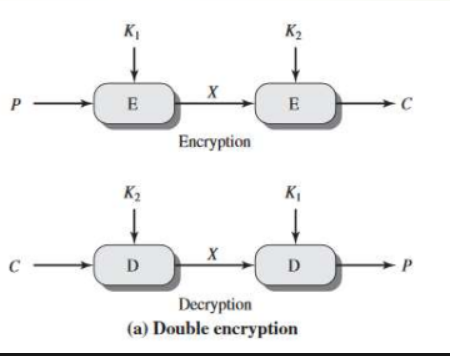
\includegraphics[width=0.4\textwidth]{img3.1.PNG} % Replace "your_image_filename" with the actual filename of your image
    \caption{} % Leave the caption empty if you don't want a label
\end{figure}

\section*{Meet-in-the-Middle Attack:}

The meet-in-the-middle attack is a cryptographic technique that takes advantage of the inefficiency in searching through the entire key space in a double encryption scenario. This method becomes particularly relevant in the context of multiple encryptions, as seen in Double DES.

Consider the Double DES scenario with two encryption keys \(K_1\) and \(K_2\):
\begin{enumerate}
    \item \(M \rightarrow \text{DES}(M, K_1) = C_1\)
    \item \(C_1 \rightarrow \text{DES}(C_1, K_2) = C_2\)
\end{enumerate}

To execute the meet-in-the-middle attack:
\begin{enumerate}
    \item Encrypt the plaintext \(M\) using all possible keys \(K_i\), storing the intermediate results: \(C = \text{DES}(M, K_i)\).
    \item Decrypt the ciphertext \(C_2\) using all possible keys \(K_2\), storing the intermediate results: \(C' = \text{DES}^{-1}(C_2, K_2)\).
    \item Compare the lists of intermediate results. If there is a match between \(C\) and \(C'\), the corresponding keys \(K_i\) and \(K_2\) can be considered as potential candidates for the correct keys used in the Double DES encryption.
\end{enumerate}

The meet-in-the-middle attack significantly reduces the effective key space from \(2^{256} \times 2^{256}\) to \(2^{256} + 2^{256}\), making it more feasible than a complete brute-force search.




\begin{figure}
    \centering
    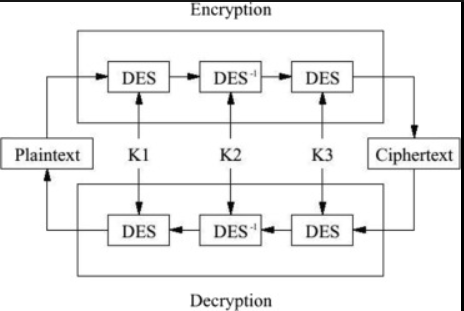
\includegraphics[width=0.4\textwidth]{img3.2.PNG} % Replace "your_image_filename" with the actual filename of your image
    \caption{} % Leave the caption empty if you don't want a label
\end{figure}


\section*{2.3 Triple DES}

Triple DES, also known as 3DES or TDEA (Triple Data Encryption Algorithm), is an important encryption algorithm that uses the Triple Data Encryption Standard (DES) cipher for security.

\subsection*{2.3.1 Encryption:}
To encrypt a plaintext \(P\) using Triple DES, denoted as \(C = \text{3DES}(P, K_1, K_2, K_3)\), the algorithm follows these steps:
\[ C = \text{DES}(P, K_1) \oplus \text{DES}^{-1}(\text{DES}(P, K_2), K_3) \]
Here, \(K_1\), \(K_2\), and \(K_3\) are three distinct 56-bit DES keys.

\subsection*{2.3.2 Decryption:}
To decrypt a ciphertext \(C\) using Triple DES, denoted as \(P = \text{3DES}^{-1}(C, K_1, K_2, K_3)\), the algorithm follows these steps:
\[ P = \text{DES}^{-1}(\text{DES}(C, K_3), K_2) \oplus \text{DES}(C, K_1) \]

Triple DES provides greater security than single DES and is widely used in many security applications.


\section*{Groups}

A \textit{group} $(G, \ast)$ consists of a set $G$ with a binary operation $\ast$ on $G$ satisfying three axioms:

\begin{enumerate}
    \item \textbf{Associativity:} $(a \ast b) \ast c = a \ast (b \ast c)$ for all $a, b, c \in G$.
    \item \textbf{Identity Element:} There exists an element $1 \in G$ called the identity element such that $a \ast 1 = 1 \ast a = a$ for all $a \in G$.
    \item \textbf{Inverse Element:} For each $a \in G$, there exists an element $a^{-1} \in G$ called the inverse of $a$ such that $a \ast a^{-1} = a^{-1} \ast a = 1$ for all $a \in G$.
\end{enumerate}

A group $G$ is abelian (or commutative) if $a \ast b = b \ast a$ for all $a, b \in G$.

\section*{Example of a Group}

Consider the set of integers $\mathbb{Z}$ with the operation of addition $+$. This forms a group because:

\begin{enumerate}
    \item \textbf{Closure:} The sum of any two integers is also an integer.
    \item \textbf{Associativity:} The addition of integers is associative.
    \item \textbf{Identity Element:} The identity element is $0$ because $a + 0 = 0 + a = a$ for all $a \in \mathbb{Z}$.
    \item \textbf{Inverse Element:} The inverse of any integer $a$ is its negation $-a$ because $a + (-a) = (-a) + a = 0$ for all $a \in \mathbb{Z}$.
\end{enumerate}

\section*{Group Operations}

Common group operations include addition, multiplication, modular arithmetic, matrix multiplication, and permutation composition. The specific operation depends on the set of elements under consideration. The key is that the operation must satisfy the group axioms.





\end{document}